\section{Introduction}\label{sec:introduction}

Software volume in vehicles has been keeping increasing for years; it is expected to increase by 50\% by 2020~\cite{ll}. 80\%
to 90\% of the innovation within the automotive industry is
based on electronics, and a big part of electronics is software~\cite{Knauss2016}.
%In line with the trend of increasing software volume in vehicles, 
The increasing complexity of software causes an increasing request for robustness. According to some reports, software errors led to almost 60-70\% of all the recalls of vehicles in Europe and North America~\cite{ll}. These errors might endanger people's life, affect manufacturers' reputation and lead to enormous economic losses. 

%The robustness of the embedded software of the vehicle is just part of the quality requirements for the vehicle embedded system. 
To increase the quality and the efficiency %for high quality and high development efficiency 
of the embedded system of the vehicle, many large manufacturers and suppliers in the automotive industry in Europe have been joined up to establish a shared standard for vehicle system architecture since 2003. The output for this effort is AUTOSAR (Automotive Open System Architecture - {\small \url{https://www.autosar.org/}}). %was put forward. 
%Automotive Open System Architecture (AUTOSAR) was defined by several large manufacturers and suppliers in the automotive industry around the world, in order for high quality and high development efficiency of the vehicle embedded software.
Its goal is to get a de-facto open industry standard for automotive E/E architectures~\cite{aa}, by which automotive systems can get better modularity, scalability, transferability and re-usability. Since then, AUTOSAR has been a popular open standard in the automotive industry. 
% because of its great value and development potential. More and more manufacturers and suppliers join and become partners of this project~\cite{ee}. 
%
%\begin{figure*}[bht]
%\centering
%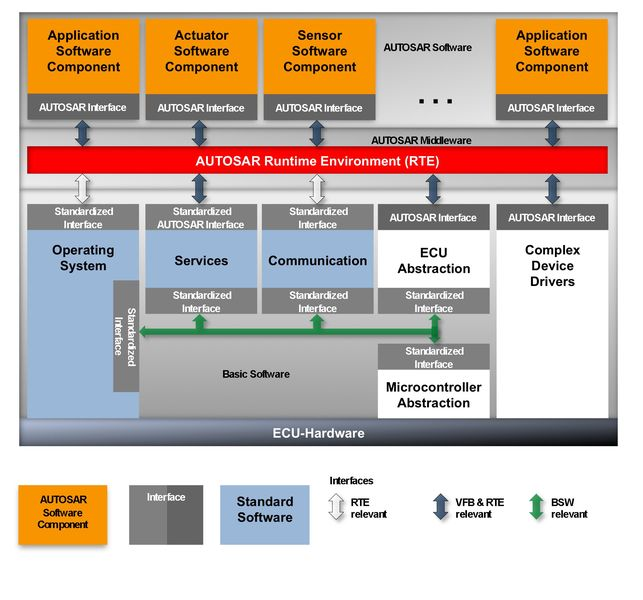
\includegraphics[width=.8\textwidth]{figure/layers_original.jpg}
%\caption{The layers of AUTOSAR architecture for an ECU (taken from~\cite{aa})}
%\label{fig:autosar}
%\end{figure*} 
%
However, %challenges also come with the popularity of AUTOSAR. As 
AUTOSAR just defines the architecture of the vehicle software system, while the implementation of the functionality is done by the manufacturers and suppliers themselves. Moreover, it is in general quite difficult to ensure that the quality expectations are met. %of which the quality is hard to ensure. 
This includes the %brings great challenges on the 
robustness of the developed AUTOSAR software components. %they developed. 
%AUTOSAR is mature, but such AUTOSAR software still needs to be improved. Researchers and developers are always willing to develop AUTOSAR software components with good robustness, they have been trying many different design ideas for development. 

In this paper we describe an industrial investigation made within Volvo AB in Gothenburg about using %made within 
Design by Contract (DbC) as a means for improving the robustness of AUTOSAR software components. 
%looks like a promising %may be a good design 
%design idea for AUTOSAR software components. %As anticipated in Section~\ref{sec:background}, i
In DbC, the relationship between a class and its clients is viewed as a formal agreement in which each party's right and obligations are described~\cite{jj}. In practice, it sets precise conditions to both the input and output of the components. %As the definition of robustness is ``the degree to which a system or component can function correctly in the presence of invalid inputs or stressful environmental conditions''~\cite{cc}. \
Since the output of one component is often the input of another component, this enables to check that the communication among components is correct. DbC helps both checking the correctness of input and output of one software component, and %. Also, it checks 
the preservation of invariants inside the software component. %To achieve a high degree of robustness, Design by Contract is worth a try. The aim of this thesis is to answer the research question:
%
%\begin{itemize}
% \item \textbf{Is the use of Design by Contract a methodology to increase the robustness of AUTOSAR software components?}
%\end{itemize}


%The work in this thesis addresses this question. I apply 
The proposed approach is implemented and applied to the components of two AUTOSAR applications. %: Brake-Lighting and Brake-By-Wire (these two components are described in Section~\ref{sec:example}). 
%In line with the %With the design 
%idea of Design by Contract, conditions for input and output are set for the Brake-Pedal-Input-Handler component in the Brake-By-Wire system and the Brake-Light-Control component in the Brake-Lighting application. %As the Brake-Pedal-Input-Handler component is also used in the Brake-Lighting application, the connection of these two components is also considered and implemented. 
The output of our approach is a set of components enhanced with contracts. These  components %which are modified with input and output checking, 
are then tested by black-box testing with ARUnit testing tool. By comparing the test results of the original and modified components, we can conclude saying that DbC greatly increases the robustness of AUTOSAR software components. In the paper we also identify and discuss limitations and weaknesses of the proposed approach.

The paper is structured as follows: Section~\ref{sec:background} provides background information that is needed to understand the approach. Section~\ref{sec:approach} presents the approach and Section~\ref{sec:implementation} describes its implementation. The validation of the approach is discussed in Section~\ref{sec:evaluation}. Related works are discussed in Section~\ref{sec:relatedWorks}. The paper concludes with final remarks and future research directions in Section~\ref{sec:conclusions}.


%the answer to the research question can be gotten.